\documentclass[english, 11pt, titlepage]{article}

\usepackage[utf8]{inputenc}    
\usepackage[english]{babel}
\usepackage[top=2.5cm, bottom=2.5cm, left=2.5cm, right=2.5cm]{geometry}
\usepackage{fancyhdr}
\usepackage{lastpage}

%Path relative to the .tex file containing the \includegraphics command
\usepackage{graphicx}
\graphicspath{ {images/} }

\pagestyle{fancy}
\fancyhf{}
\rhead{(\thepage)}
\lhead{LP2A - Spring 2021}

% Clickable table of contents
\usepackage{hyperref}
\hypersetup{
    colorlinks,
    citecolor=black,
    filecolor=black,
    linkcolor=black,
    urlcolor=black
}

\begin{document}

    \begin{titlepage}
    \begin{center}
        \vspace*{1cm}
            
        \Huge
        \textbf{Programming a Ludo Game}
            
        \vspace{0.5cm}
        \LARGE
        Project report
            
        \vspace{1.5cm}
            
        \textbf{Florian CLOAREC} \\
        \textbf{Théo DURR}
        
        \vspace{1.5cm}
        
        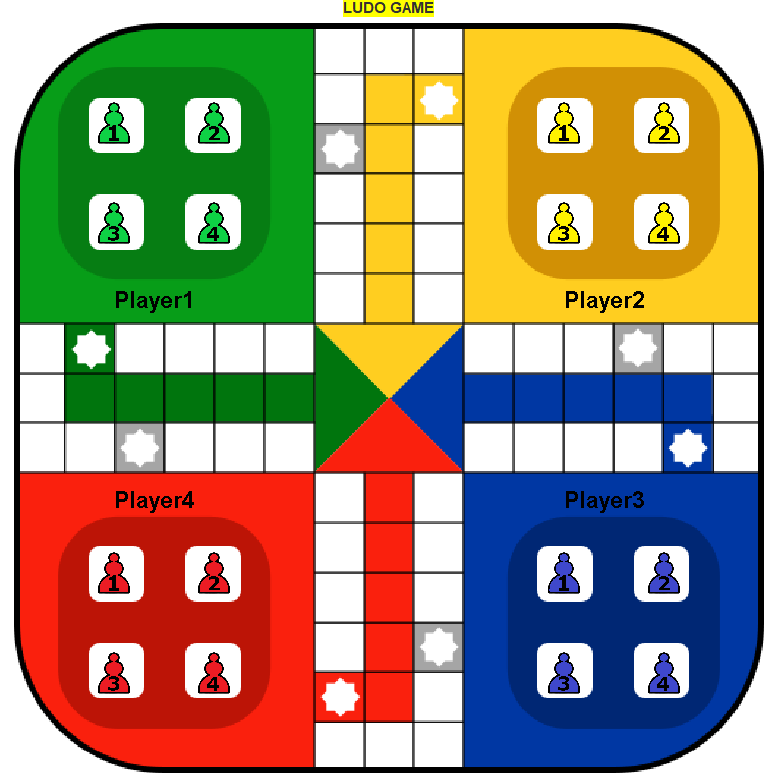
\includegraphics[width=0.45\textwidth]{titlepage.jpg}

        \vfill
                  
        
        \Large
        LP2A - Introduction to object conception and programming \\
        Spring 2021\\
        Université de Technologie de Belfort-Montbéliard\\
        \vspace{0.5cm}
        
\includegraphics[width=0.3\textwidth]{utbm_forword-2.jpg}
            
    \end{center}
\end{titlepage}

    \pagebreak
    \tableofcontents

    \pagebreak
    \section{Introduction}
    \subsection{Project Analysis}
    % Talk about UML, OOP programming
    First of all, we performed an analysis of the subject by defining, the behaviour, the constraints or even the signature of each class and represented all of this in an \textbf{UML Class Diagram}.
    \subsection{Organization}
    % Talk about task repartition
    % Talk about git, IntelliJ
    We also used some tools like IntelliJ Idea as IDE, for time saving tasks like compiling, creating packages, making unit tests, and so on. As a \textbf{Version Control System (VCS)}, we used \emph{Git}

    \section{The game components}
    This project is split into two main components : \emph{game engines} and \emph{graphical user interface (GUI)}. The engines are the core of the game. They ensure IAs are following certain rules, as well as player, who are restricted in their choices with the GUI by displaying only "rules friendly" moves. We will detail some of the functionnalities.

    Before explaining the engines, we need to talk about the components needed for it. They play a main role in the OOP. Yet, they are quite simple. For a summarized view of the structure, see APPENDIX X

    \subsection{The Player}
    \subsubsection{Human}

    \subsubsection{Artificial Intelligence}

    \subsection{The Coordinates System}

    \subsection{The board}

    \section{The game engines}
    They are 3 engines in total. Each engine is called depending of the gamemode. By following OOP principles, all the engines inherit from an abstract parent class called \verb|Engine|.

    \subsection{4 Artificial Intelligences}
    This gamemode was not required in the specifications, but we made it for \emph{experimental purposes}. It allowed us to check if everything was working properly without having a GUI. The four players are AIs and are playing by following the rules.
    \subsection{4 Players}
    This gamemode unlieve the entire potential of the GUI, by allowing four players to play in the same time on the same computer. Each player plays one after the other.

    \subsection{1 Player versus 3 Artificial Intelligences}

    \section{The graphical user interface (GUI)}
    \subsection{Translating relatives coordinates in absolute coordinates}
    
\end{document}